\subsection{Mecanismos de transferencia de energía en procesos térmicos}

  \PN El proceso de transferencia de energía por calor también se llama \textbf{conducción} o \textbf{conducción
  térmica}.

  \vspace{3mm}
  \PN Consideremos el siguiente modelo:
  \begin{figure}[H]
  \centering
    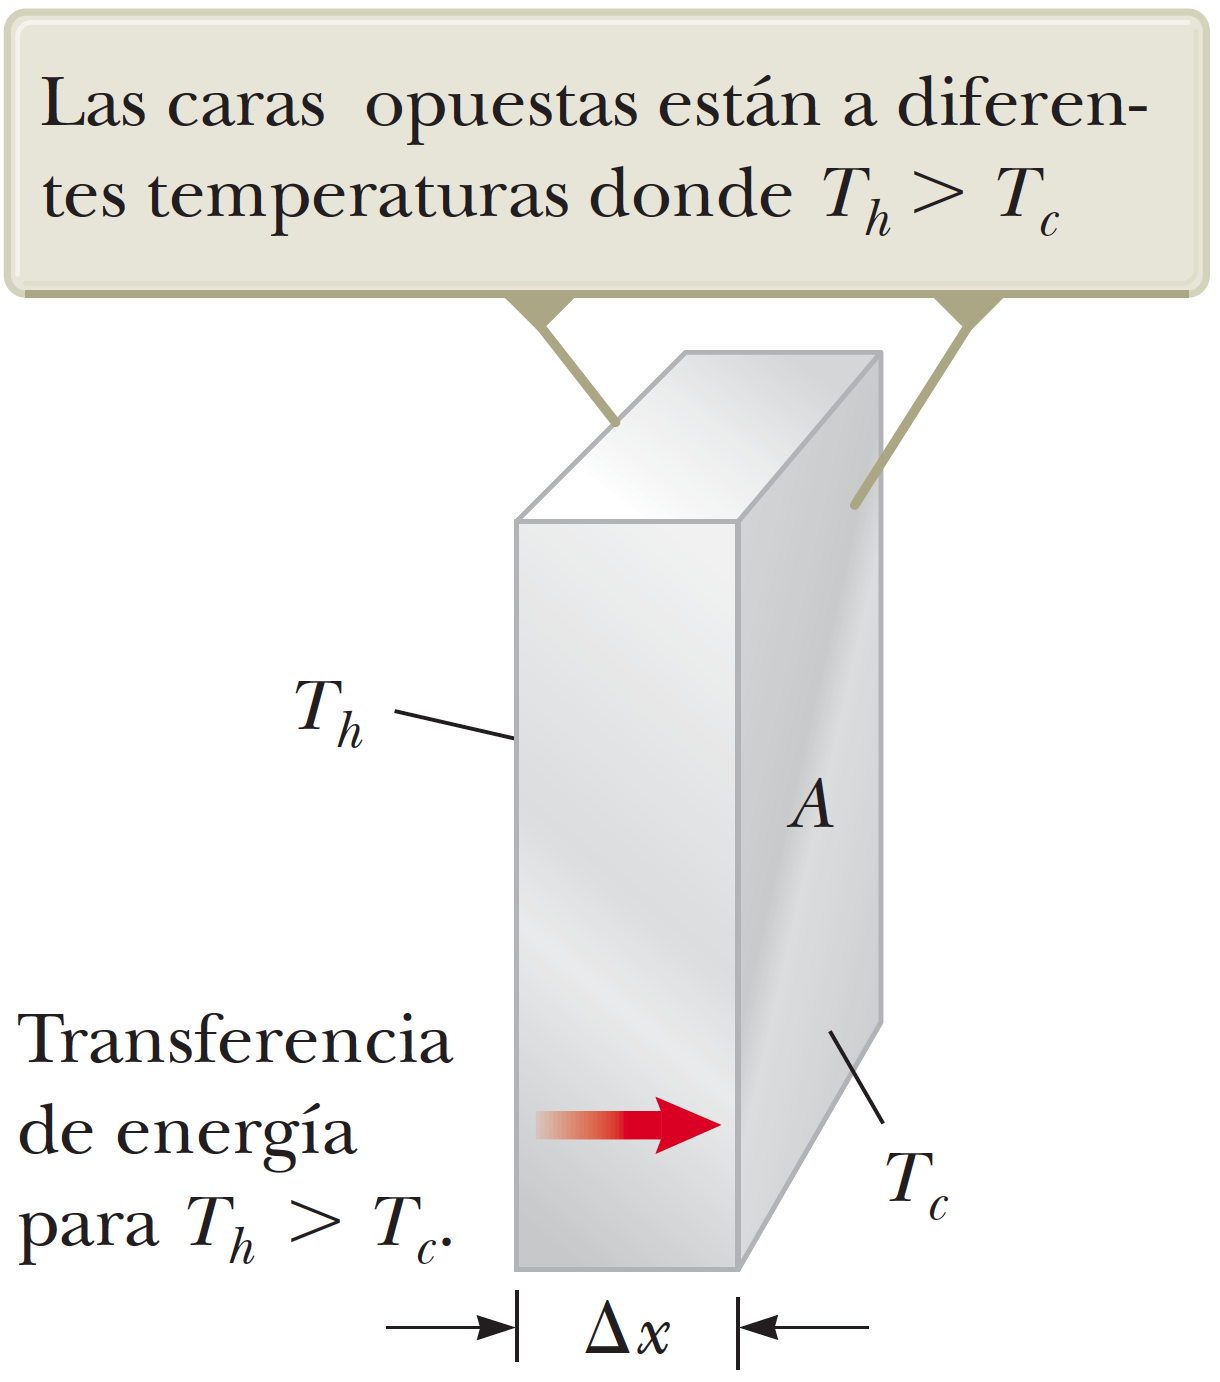
\includegraphics[width=0.3\textwidth]{3/figure_1}
    \caption{Transferencia de energía a través de una placa conductora con un área de sección transversal A y un espesor
    $\Delta x$.}
  \end{figure}

  \PN La conducción se presenta sólo si hay una diferencia en temperatura entre dos partes del medio de conducción.
  Considere una placa de material de espesor $\Delta x$ y área de sección transversal A. Una cara de la placa está a una
  temperatura $T_{c}$ y la otra está a una temperatura $T_{h} > T_{c}$. Se encuentra que la energía Q se transfiere en
  un intervalo de tiempo $\Delta t$ desde la cara más caliente hacia la más fría. La rapidez $P = \text{Q} / \Delta t$ a
  la que ocurre esta transferencia de energía se encuentra que es proporcional al área de sección transversal y a la
  diferencia de temperatura $\Delta T = T_{h} - T_{c}$, e inversamente proporcional al espesor:
  \begin{equation*}
    \text{P} = \frac{\text{Q}}{\Delta t} \propto \text{A} \frac{\Delta \text{T}}{\Delta x}
  \end{equation*}

  \PN Para una placa de espesor infinitesimal $dx$ y diferencia de temperatura $dT$, se escribe la \textbf{ley de
  conducción térmica} como:
  \begin{equation*}
    \text{P} = k \text{A} \abs{\frac{d\text{T}}{dx}}
  \end{equation*}

  \PN donde la constante de proporcionalidad $k$ es la conductividad térmica del material y $\abs{\frac{dT}{dx}}$ es el
  gradiente de temperatura.

  \vspace{3mm}
  \PN Suponga que una larga barra uniforme de longitud L se aísla térmicamente de modo que la energía no puede escapar
  por calor de su superficie, excepto en los extremos. Un extremo está en contacto térmico con un depósito de energía a
  temperatura $T_{c}$, y el otro extremo está en contacto térmico con un depósito a temperatura $T_{h} > T_{c}$. Cuando
  se logra un estado estable, la temperatura en cada punto a lo largo de la barra es constante en el tiempo. En este
  caso, si se supone que $k$ no es una función de la temperatura, el gradiente de temperatura es el mismo en todas
  partes a lo largo de la barra y es:
  \begin{equation*}
    \abs{\frac{d\text{T}}{dx}} = \frac{\text{T}_{h} - \text{T}_{c}}{\text{L}}
  \end{equation*}

  \PN Por lo tanto, la rapidez de transferencia de energía por conducción a través de la barra es:
  \begin{equation*}
    \text{P} = \frac{k\text{A}}{\text{L}} \left(\text{T}_{h} - \text{T}_{c}\right)
  \end{equation*}

  \PN \textbf{Resistencia térmica}
  \PN El término L/$k$ para una sustancia particular se conoce como el valor R del material. Por lo tanto
  \begin{equation*}
    \text{P} = \frac{\text{A} \left(\text{T}_{h} - \text{T}_{c}\right)}{\sum_{i} R_{i}}
  \end{equation*}

  \PN donde $R_{i} = \text{L}_{i} / k_{i}$.

  \vspace{3mm}
  \PN \textbf{Convección}
  \PN Se dice que la energía transferida por el movimiento de una sustancia caliente se transfiere por convección, que
  es una forma de transferencia de materia.
  \begin{equation*}
    \text{P} = h \text{A} \left(\text{T} - \text{T}_{0}\right)
  \end{equation*}

  \PN donde $h$ es la \textit{constante de convección}, A es la \textit{superficie de contacto} y T es la
  \textit{temperatura del cuerpo}.

  \vspace{3mm}
  \PN \textbf{Radiación}
  \PN El tercer medio de transferencia de energía que se analizará es la \textbf{radiación térmica}.
  \PN La rapidez a la que un objeto radia energía es proporcional a la cuarta potencia de la temperatura absoluta de la
  superficie. Conocida como ley de Stefan, este comportamiento se expresa en forma de ecuación como:
  \begin{equation*}
    \text{P} = \sigma \text{A} e \text{T}^{4}
  \end{equation*}

  \PN donde P es la potencia en watts de las ondas electromagnéticas radiadas de la superficie del objeto, $\sigma$ es
  una constante igual a $5.67$ x $10^{-8} \; W/m^{2} K^{4}$, A es el área superficial del objeto en metros cuadrados,
  $e$ es la emisividad y T es la temperatura superficial en kelvins.

  \PN Si un objeto está a una temperatura T y sus alrededores están a una temperatura promedio T$_{0}$, la rapidez neta
  de energía ganada o perdida por el objeto como resultado de la radiación es:
  \begin{equation*}
    \text{P}_{neta} = \sigma \text{A} e \left(\text{T}^{4} - \text{T}_{0}^{4}\right)
  \end{equation*}
